
\chapter*{Введение}
\addcontentsline{toc}{chapter}{Введение}
\hspace{1cm} Независимо от стараний разработчика или сложности проекта, большая часть времени разработки
будет потрачена на то, чтобы убедиться, что устройство работает правильно, или -- что наиболее
вероятно -- разобраться, почему устройство работает не так, как ожидалось. Отладчик -- самый мощный 
инструмент в наборе инструментов разработчика, позволяющий напрямую взаимодействовать с процессором,
задавать точки останова, пошагово управлять потоком выполнения инструкций и проверять  значения
регистров. \cite{Lakamera:embed}

Для устройств <<Интернета вещей>> очень важно знать и отслеживать энергопотребление,
ведь обычно такие устройства питаются от батарейки и каждое ненужное действие уменьшит
срок службы. Мониторинг энергопотребления позволяет понять энергоэффективность каждого сеанса связи,
что позволит выбрать наиболее подходящий интерфейс и протокол передачи данных.

Об актуальности возможности мониторинга энергопотребления для отладчика говорит количество 
измерительных устройств на рынке. Характеристики основных из них приведены в таблице 
\ref{comparemeasdevices}.

\begin{table}[H]
    \caption{Сравнение характеристик измерительных устройств}
    \label{comparemeasdevices}   
    \begin{center}
    \begin{tabular}{|c|c|c|c|c|}
    \hline
  Устройство & Joulescope & Otii Arc & NanoRanger & Current Ranger \\ \hline
    Диапазон тока & от -1 А до 3 А & от 0 до 2,5 А & от 1 нА до 800 мА & от -1,65 А до 3 А \\ \hline
    Разрешение & 1 нА & десятки нА & до 10 пА & до 1 пА  \\ \hline
    Погрешность & до 0,3\% & до 0,1\% & до 0,3\% & до 0,1\% \\ \hline
    Цена & 800 \$ & 700 \$ & 220 \$ & 120 \$  \\ \hline
    \end{tabular}
    \end{center}
\end{table} 

Так же о высокой потребности в устройстве говорит большое количество существующих отладчиков с 
мониторингом энергопотребления от различных производителей микроконтроллеров, например STLINK-V3 
\cite{STLINKV3} и Power Profiler Kit II \cite{Power Profiler Kit}, так и от сторонних компаний, например 
Energymon.

Хорошим примером, где активно используются подобные отладчики является французская FIT IoT-LAB. 
Это группа удаленных лабораторий, которые предназначены для проведения массовых экспериментов 
с устройствами интернета вещей, и имеют открытый исходный код и свободный доступ по всему миру.
FIT IoT-LAB имеют шесть площадок, поддержку 18 популярных аппаратных платформ. 
Каждая лаборатория состоит из набора отладчиков, которые реализуют общение с сервером, заливку прошивки
и другие функции, с подключаемыми к ним отладочными платами. Из недостатков французского решения стоит 
отметить реализацию каждого отладчика на PaspBerry, что довольно дорого, и скудные возможности мониторинга 
энергопотребления.

В МИЭМ начинает свою работу подобная лаборатория MIEM IoT-LAB, которая имеет потребность в удаленном
отладчике, а также в возможности мониторинга энергопотребления отлаживаемых устройств, 
как как это сделано в оригинале у FIT IoT-LAB, а так же улучшение французского решения в сторону 
замены аппаратной реализации с PaspBerry на микроконтроллер и повышения 
точности и качества мониторинга потребляемой мощности у отлаживаемых устройств. \cite{FITIoT}.

Так как разрабатываемое устройство является отладчиком, то для <<общения>> с отлаживаемым устройством 
в отладчике должны быть реализованы стандартные для этих целей интерфейсы, такие как UART и отладочные 
SWD/JTAG, что подразумевает под собой наличие удобных, распространенных разъемов. Также, из-за планируемого 
использования в MIEM IoT-LAB, отладчик должен уметь общаться с <<сервером>> по Ethernet, что, по сути,
является требованием заказчика, обусловленное потребностью в возможности гибкого размещения лаборатории на 
территории МИЭМа.

Определяя требования к диапазонам измеряемого тока, стоит учитывать различные IoT-устройства. Грубую оценку
можно составить на примере Wi-Fi решений и сотовых модемов, которые в <<пике>> передачи данных могут 
иметь потребление в районе одного ампера, а в спящем режиме потребляют порядка единиц мкА.

%ссылку на инфу

Перед проектированием отладчика с возможностью мониторинга энергопотребления IoT-устройств
следует определиться с требованиями, предъявляемыми к отладчику. 
Для этого в качестве примера рассмотрим <<усредненный>> паттерн поведения устройства с BLE, одной
из самых популярных технологий беспроводной передачи данных интернета вещей, 
у которого с периодичностью в несколько десятков мс повторяется такой цикл: спящий режим 
с токопотреблением единицы мкА, далее устройство просыпается, в этот момент
энерго потребление составляет единицы мА, время просыпания -- десятки мкс, далее происходит
сеанс связи, который начинается с передачи, с токопотреблением примерно десятки мА 
и длительностью передачи <<пустого>> пакета величиной 27 байт около 200 мкс, и продолжается 
ожиданием ответа длительностью в среднем 150 мкс, после сеанс связи завершается приемом,
при котором токопотребление составляет единицы-десятки мА длительностью 200 мкс.

Зная ориентировочные диапазоны измеряемых токов, можно промоделировать данный паттерн 
поведения BLE-устройства в LTSpice, чтобы грубо оценить необходимую полосу пропускания отладчика. 
Моделируемая схема представлена на рисунке \ref{ris:LTSpiceScheme}, результаты моделирования 
представлены на рисунках \ref{ris:LTSpice0_01} - \ref{ris:LTSpice100} и имеют больше 
демонстрационно-оценочный характер.

\begin{figure}[H]
  \centering
  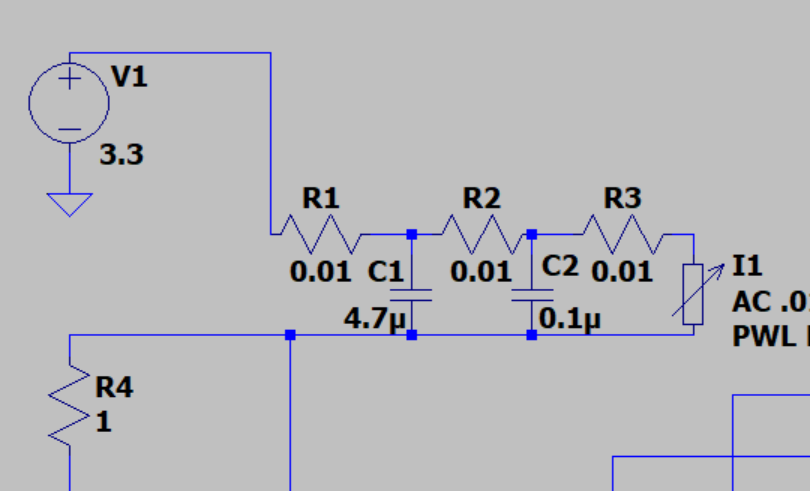
\includegraphics[scale = 0.5]{LPSpice scheme.png}
  \caption{Моделируемая схема}
  \label{ris:LTSpiceScheme}
\end{figure}

\begin{figure}[H]
  \centering
  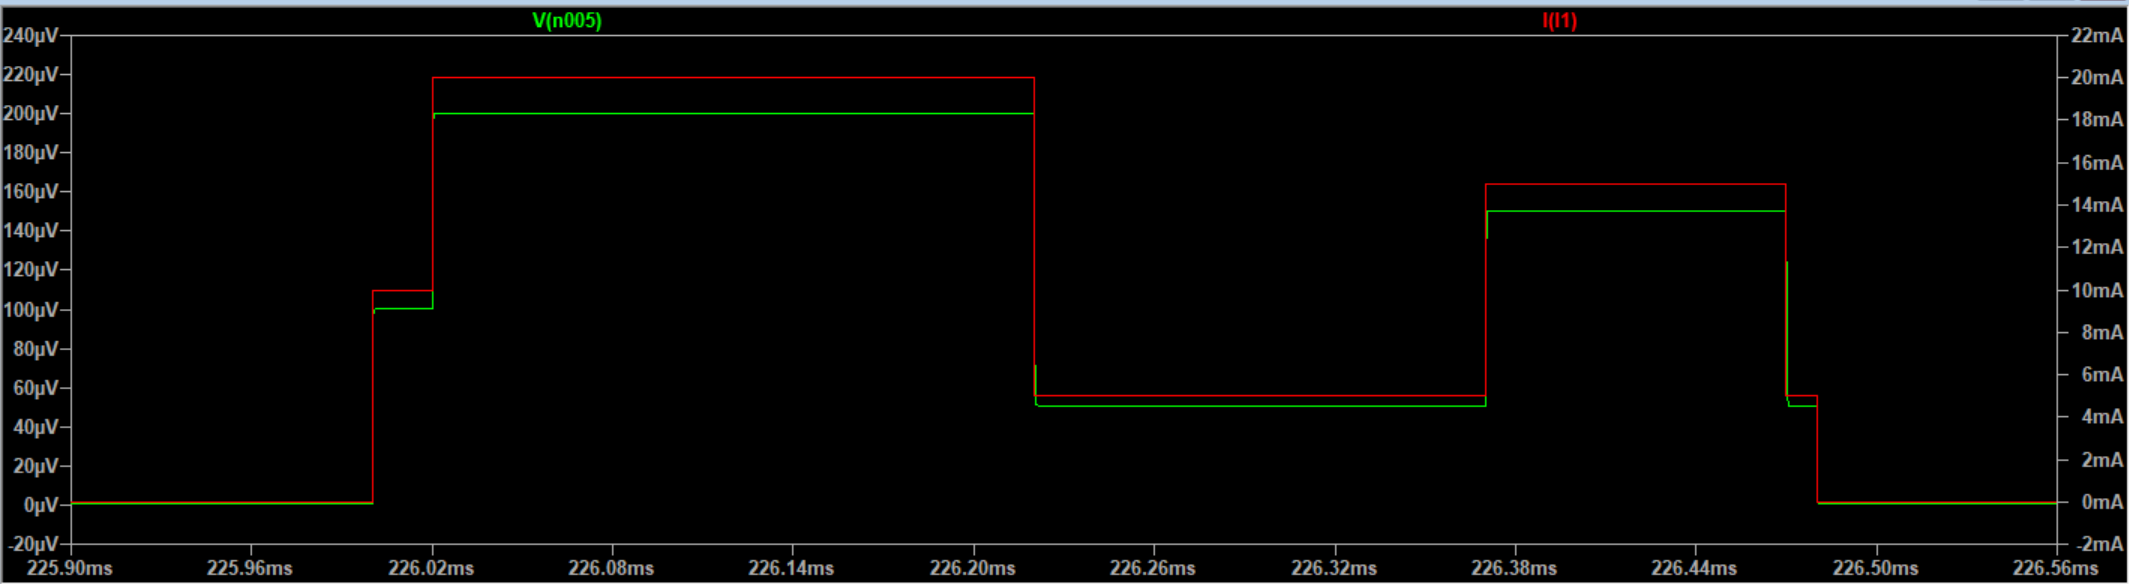
\includegraphics[scale = 0.3]{LTSpice0_01.png}
  \caption{Результаты моделирования амперного диапазона }
  \label{ris:LTSpice0_01}
\end{figure}

Резисторы R1 -- R3 моделируют сопротивления проводников на печатной плате, конденсаторы C1 -- C2 фильтрующие 
по питанию, I1 -- источник тока, моделирующий вышеописанный паттерн поведения BLE-устройства,
R4 - шунт, для амперного диапазона, который равен 0,01 Ом (в дальнейшем в ходе дипломной работы уточняется). 
Красная линия -- входной сигнал, моделирующий потребление отлаживаемого устройства, 
зеленная -- падение напряжения на измеряемом шунте. 

\begin{figure}[H]
  \centering
  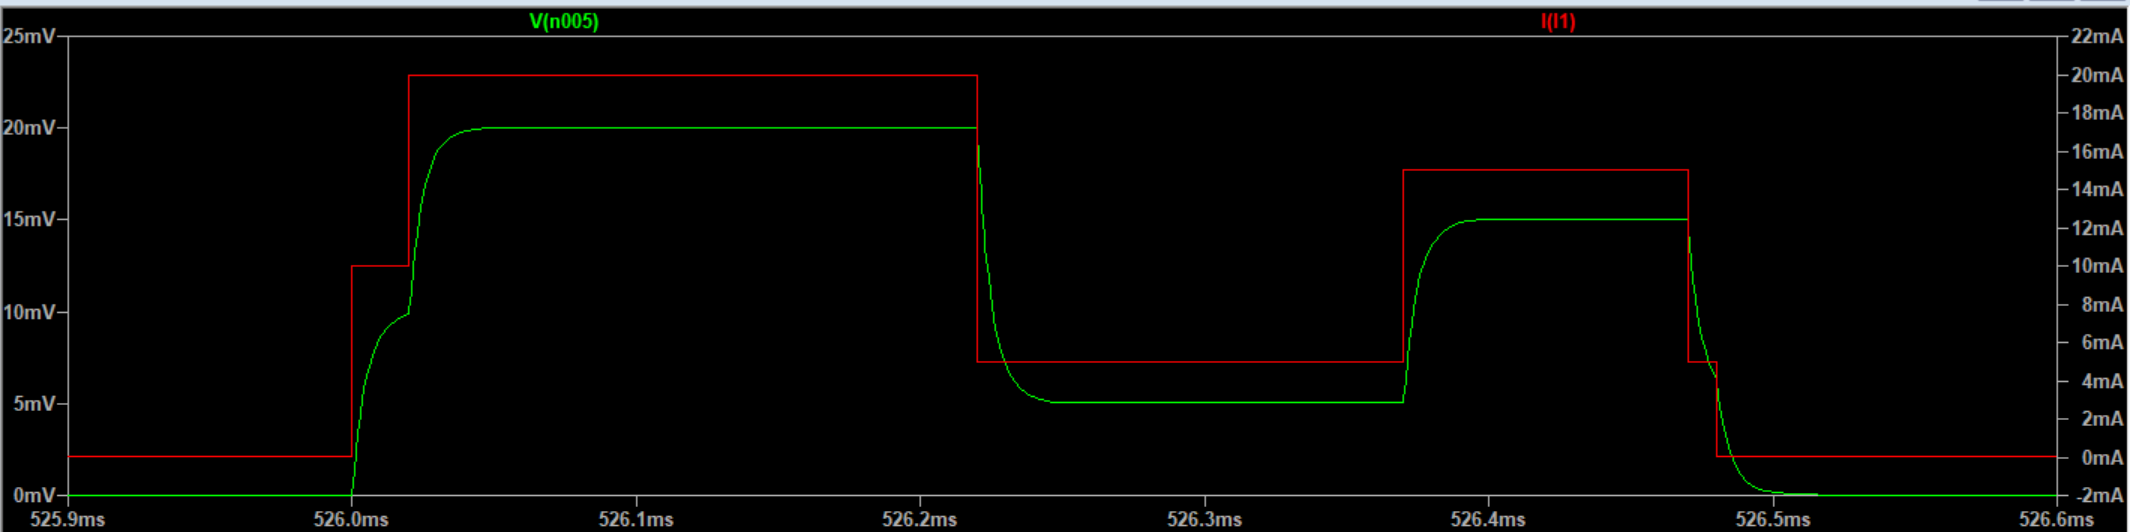
\includegraphics[scale = 0.3]{LTSpice_1.png}
  \caption{Результаты моделирования миллиамперного диапазона }
  \label{ris:LTSpice_1}
\end{figure}

Здесь шунт R4 равен 1 Ом, диапазон -- миллиамперный. 

\begin{figure}[H]
  \centering
  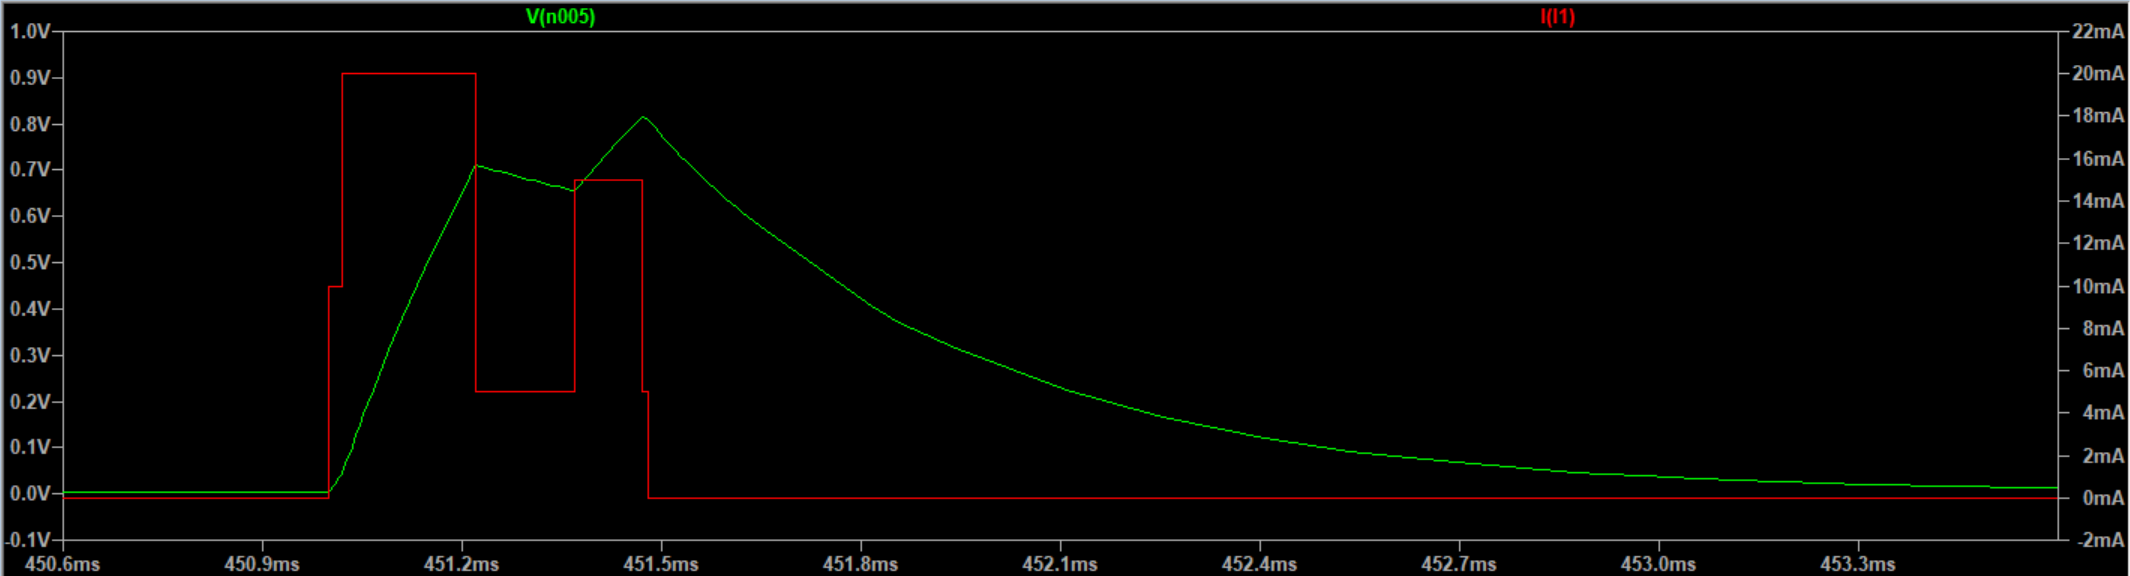
\includegraphics[scale = 0.3]{LTspice100.png}
  \caption{Результаты моделирования микроамперного диапазона }
  \label{ris:LTSpice100}
\end{figure}

А вот моделирование микроамперного диапазона, который можно считать основным измерительным диапазоном для 
IoT-устройств с малым энергопотреблением, показывает, что из-за получившегося из R1 -- R3 и C1 -- C2 RC-фильтра,
уменьшение полосы пропускания на порядки до, примерно, значения в 15 кГц, что определяет минимальное
требование к полосе пропускания микроамперного диапазона. 
  

Для обеспечения конкурентноспособности отладчика, остальные характеристики можно определить 
из таблицы \ref{comparemeasdevices}, а так же из анализа типичной используемой элементной базы.

Резюмируя вышесказанное, можно ориентироваться на следующие требования к разрабатываемому 
устройству:
\begin{itemize}
    \item полоса пропускания -- 15 кГц для микроамперного диапазона и 50 кГц для миллиамперного и 
    амперного диапазонов
    \item напряжение питания отлаживаемых устройств -- от 1,8 В до 12 В
    \item погрешность измерения -- до 5\%
    \item диапазон тока -- от 3,2 мА до 2 А
    \item время переключения диапазонов 5 -- 10 мкс
    \item поддержка Ethernet со стороны ведущего устройства и UART, SWD/JTAG со стороны отлаживаемых
    устройств.
\end{itemize}

Данные требования, предъявляемые на этапе начального анализа, в ходе более детальной проработки,
изучения и тестирования в дальнейшем будут уточнены в соответствии с полученными результатами.
